\subsection{Propuesta de diseño}
\label{propuesta}

\textit{Deberíamos incluir el gráfico que utiliza los elementos de REST para definir la arquitectura. Justificar por punto del objetivo el diseño propuesto.}\\

\todo{Se puede agregar algo referente al patrón Microservices Architecture Pattern http://www.oreilly.com/programming/free/files/software-architecture-patterns.pdf}

% ver en http://www.oreilly.com/programming/free/open-by-design.csp?download=yes&order=574386
% se puede sacar algo referente al opensource
% otro que puede servir Migrating to the Cloud?

Por lo expuesto anteriormente, se propone una arquitectura más desacoplada a la planteada con el \textit{Integrador}, permitiendo de esta manera minimizar el costo del mantenimiento, desarrollo y simplificando el deployment en entornos de producción.  Una solución basada en estándares que permita integrar sistemas heterogéneos, aceptando el hecho de que la mayoría de los sistemas legados que se encuentran en producción, se mantendrán y logrando de esta manera, que la infraestructura subyasente facilite la incorporación de cambios que puedan surgir como necesidades de la organización.

La estrategia de orientación a servicios permite la creación de servicios y aplicaciones compuestas que pueden existir con independencia de la tecnologías subyacentes\cite{microsoft2006}.

El modelo de servicios facilita el acceso y consumo de la información a traves de la red.  Dado que los servicios son independientes y autónomos, pueden combinarse tantas veces como sean necesarias de manera sencilla, generando nuevas aplicaciones que respondan a las necesidades cambiantes de la organización.

El resultado final es una organización que se adapta fácilmente a los cambios, creando y reutilizando servicios y aplicaciones...


\subsubsection{Desacoplamiento}

Para lograr el desacoplamiento, primero se deberá desarrollar una \textit{API de Referencias}, en la cual se implementarán los servicios necesarios que permitirán el acceso a los datos de referencia desde las distintas aplicaciones.  El acceso a la \gls{acro:api}, estará restringido a las direcciones IP de las aplicaciones (clientes) y al uso de un token, que se utilizará para validar el acceso a los servicios.  Esta funcionalidad no será necesario desarrollarla, ya que esta capa de seguridad se implementará mediante el \gls{acro:esb}.

Para la solución planteada, podemos observar las siguientes ventajas:

\begin{itemize}
  \item Escalabilidad: permite escalar horizontalmente, es decir, en el hipotético caso que la \textit{API de Referencias} sea accedida por muchas aplicaciones, la misma podría replicarse en varias instancias, evitando la sobrecarga de cualquiera de ellas, al mismo tiempo que serviría como failover.  Más adelante trataremos el tema de caching y balanceo.

  \item Administración centralizada: se centraliza la administración de los datos de referencia, evitando que la duplicidad se propague en cada aplicación que necesite utilizarlos.  Un ejemplo de datos de referencia puede ser el Tipo de Documento (DNI, LC, LE, etc).

  \item Mantenimiento centralizado: cuando hablamos de mantenimiento nos referimos a mejoras en la \gls{acro:api}, como por ejemplo, implementación de nuevos servicios, arreglo de bugs, etc.  Tener una \textit{API de Referencias} totalmente desacoplada de las aplicaciones que generan los datos, permite actualizarla de forma más sencilla, evitando parar momentáneamente otras aplicaciones.

  \item Agilización en el desarrollo: otra de las ventajas que presenta este esquema, es la agilización en el desarrollo de nuevas aplicaciones, ya no será necesario desarrollar el módulo que administra los datos de referencia, los mismos estarán en la \textit{API de Referencias} y se accederán a través de servicios.  De esta manera, evitamos duplicar código fuente para implementar esta funcionalidad, al mismo tiempo que acortamos los tiempos de desarrollo.
\end{itemize}

En segunda instancia, se deberán re-escribir todas las \glspl{acro:api} que se encuentran actualmente en producción, esto es lo que llamaremos \textit{API de Servicios}.  Para esto, se utilizará el lenguaje de programación Ruby con el framework Sinatra, más adelante desarrollaremos el porqué del uso de estas tecnologías.  Esto dará origen a diferentes \textit{API de servicios}, que antes se encontraban implementados en cada aplicación y acopladas a la misma, ahora estarán implementados en una instancia virtual.
De esta manera desacoplamos la lógica de la aplicación del acceso a los datos que se generan en la misma, permitiendo que esta solución escale horizontalmente, al igual que la \textit{API de Referencias}.
Tambíen hay que tener en cuenta que esta solución permite independizarse del lenguaje en el que se desarrolló la aplicación, la misma puede estar escrita en PHP, pero la \gls{acro:api} en Ruby, generando así un core o capa de servicios independiente de las aplicaciones, su única dependencia radica en el modelo de datos de cada aplicación, si se modifica el modelo de la aplicación, se modifica el acceso a los datos, es decir los servicios.

\todo{Explicar pq usamos Ruby + Sinatra para las APIs}

\subsubsection{Simplicidad}

Es más simple que el anterior porque...

minimizar el costo del mantenimiento, desarrollo, testing, al mismo tiempo que se simplifica el deployment de los distintos entornos (desarrollo, testing y producción)

\subsubsection{Fault Tolerance}

Los sistemas distribuidos potencialmente tienen mas fallos que los sistemas monolíticos, en cada solicitud intervienten diez (o cientos) microservicios diferentes.\cite[p.~48]{stin2015}  Por lo tanto, no es suficiente descomponer un sistema en componentes \eng{deployables} independientes; también hay que evitar que un fallo en uno de estos componenetes, cause un fallo en cascada.\cite[p.~4]{stin2015}

Un fallo en cascada ocurre cuando un error en una capa, provoca un fallo en la capa llamada.\cite[p.~65]{nygard2007}  Mike Nygard describe en su libro ``Release It!''\cite{nygard2007}, varios patrones tolerantes a fallos, de los cuales el mas popular es \eng{circuit breaker}.

\begin{figure}
  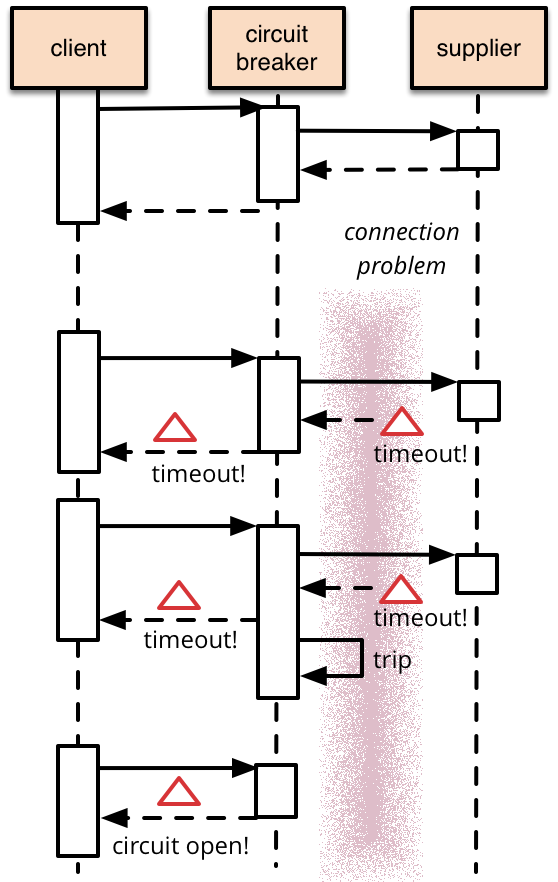
\includegraphics[width=\linewidth]{src/images/03-capitulo-3/circuit_breaker.png}
  \caption{Circuit Breaker.}
  \label{fig:circuit_breaker}
\end{figure}

Fault isolation
In order to limit the risk associated with failure, we need to limit the scope of components or features that could be affected by a failure. If no one could purchase products from Amazon.com every time the recommendations engine went down,
that would be disastrous. Monolithic application architectures often possess this type of failure mode. Cloud-native application architectures often employ microservices (“Microservices” on page 10). By composing systems from microservices, we can limit the scope of a failure in any one microservice to just that microservice, but only if combined with fault tolerance.\cite[p.~3]{stin2015}

\subsubsection{Redundancia y Escalabilidad}

\todo{antes hablar o introducir el término o patro microservices arquitecture - \url{http://microservices.io/patterns/microservices.html}}

Cuando hablamos de escalabilidad, podemos basarnos en el modelo de escalabilidad llamado \eng{scale cube}.
En este modelo, escalar aplicaciones corriendo clones detrás de un balanceador, es conocido como \eng{X-axis scaling}.  Las otras dos formas de escalar son: \eng{Y-axis scaling} y \eng{Z-axis scaling}.
En la arquitectura de microservicios, se aplica fundamentalemnte \eng{Y-axis scaling}, descomponiendo la aplicación en un conjunto de servicios colaborativos.  Cada servicio implementa un conjunto de funciones estrictamente, relacionados.\cite{website:akfpartners-scale-cube}.

\begin{figure}
  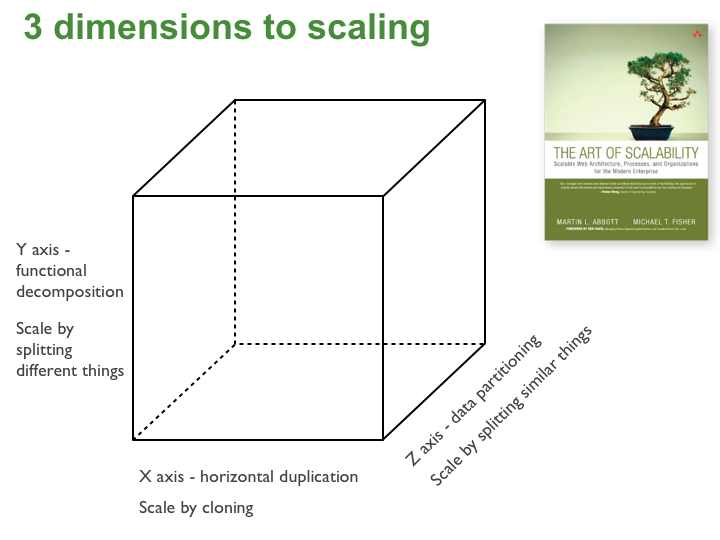
\includegraphics[width=\linewidth]{src/images/03-capitulo-3/scale_cube.jpg}
  \caption{Tres dimensiones para escalar.}
  \label{fig:scale-cube}
\end{figure}

Por lo tanto, la arquitectura de servicios debe ser replicable y escalable.  Para lograr esto, cada \gls{acro:api} correrá en una instancia virtual, la misma se replicará tantas veces como sean necesarias (\eng{X-axis scaling}).

El acceso a esta arquitectura replicada, será a través de un balanceador de carga, que servirá tanto, para balancear la carga como failover, dando continuidad a los servicios en caso de que alguna de las instancias replicadas fallen.

La característica fundamental de un balanceador de carga, es ser capaz de distribuir las peticiones entrantes, a un grupo de servidores (backends) de acuerdo a un scheduler.  Dependiendo de la complejidad del scheduler, la selección del backend podría ser aleatoria o round robin.  Algoritmos de balanceo más sofisticados, tienen en cuenta otros factores como por ej. carga del backend, tiempo de respuesta, número de conexiones activas, ubicación geográfica, etc.
En su funcionamiento básico, el balanceador redirige las peticiones a alguno de los backends, que luego contestan al balanceador, para que finalmente, sea el balanceador el que entregue la respuesta al cliente, sin que este último sepa que fue redirigido a otro servidor.  De esta manera se evitan los accesos directos desde los clientes a los servidores backends.
Como se mencionó anteriormente, el balanceador puede ser usado como failover, permitiendo la continuidad del servicio, luego del fallo de uno o más backends.  Los backends son monitoreados continuamente por el balanceador, cuando uno de estos falla, el balanceador deja de enviar tráfico al backend caído.  Luego cuando el backend vuelva a estar online, el balanceador podrá enviarle tráfico nuevamente.

Delante del balanceador, se implementará una caché compartida utilizando \gls{db:varnish}, la misma evitará los accesos al balanceador, que puedan impactar de forma directa en alguna de las instancias replicadas de la \textit{API de Servicios} y \textit{API de Referencias}.

Según la RFC 7234, una memoria cache, almacena respuestas en pos de reducir el tiempo de respuesta y el consumo del ancho de banda. Así mismo, una memoria cache compartida, es una cache que almacena respuestas para ser usadas por más de un usuario. Más adelante se tratará en detalle el uso de caches compartidas.

Como bien se indicó anteriormente, una caché compartida evitará los accesos a cualquiera de las instancias, ya sea \textit{API de Referencias} o \textit{API de Servicios}, obteniendo mejores tiempos de respuesta así como tolerancia a fallos.  Por ej. pensemos en una aplicación (cliente A) que accede al servicio de Dependencias (/dependencies) de la \textit{API de Referencias}.  La petición es atendida por la \textit{API de Referencias}, donde el servicio devuelve todas la dependencias activas, ordenadas por nombre.  Más tarde, otra aplicación (cliente B), vuelve a consultar la \gls{acro:api} por las dependencias, accediendo nuevamente al servicio /dependencies de la \textit{API de Referencias}, quien responde con el listado de dependencias ordenado por nombre.  Como se puede apreciar, tenemos dos accesos a la \textit{API de Referencias} con indénticas respuestas.  Esta situación se puede evitar con una cache compartida entre los diferentes clientes, logrando mejorar los tiempos de respuesta, ya que la \textit{API de Referencias} no debe acceder ni procesar los datos, debido a que los mismos son obtenidos desde la cache compartida.

\subsubsection{Estandarización}

Como mencionamos anteriormente, para cada aplicación se deberá implementar una \gls{acro:api} de acceso a datos propios generados localmente, esta re-escritura se realizará basándose en la especificación \gls{acro:jsonapi}, la cual se encuentra en su versión estable 1.0.
Según el diccionario de la Real Academia Española,  un estándar es lo que sirve como tipo, modelo, norma, patrón o referencia, en nuestro caso, la estandarización es el proceso por el cual se establecen normas comúnmente aceptadas que permiten la comunicación de diferentes aplicaciones.

Esta estandarización facilitará el desarrollo de clientes que consuman de los diferentes servicios de las \glspl{acro:api}, ya que contamos con reglas que especifican cómo se podrá acceder a los datos, cuál será su estructura de respuesta, incluso logramos independencia del lenguaje con el que se escriban estos clientes, quienes deben respetar las especificaciones para implementar el acceso a los servicios.

Por lo tanto, la utilización de \gls{acro:jsonapi} como estructura de intercambio e interacción \gls{acro:api} <=> Aplicación, radica en el uso de un estándar que ha alcanzado un nivel de madurez que permite hoy contar con su versión 1.0.
